\chapter{Storia della scrittura}
\section{Il filo rosso che unisce passato e presente nella scrittura}
Prendendo in considerazione l'intera storia umana, l'evoluzione, c'è un \textit{filo rosso} che unisce il modo di comunicare e scrivere dell'uomo del passato a quello attuale: \hl{la velocità/il tempo con cui l'uomo riesce ad esprimersi e archiviare informazioni}.
\\\\
Già l'uomo delle caverne, a modo suo, comunicava e scriveva qualcosa; abbiamo, ancora oggi, segni tangibili della sua esistenza e modo di comunicare graficamente attraverso la scrittura/disegno. 

Proseguendo nell'evoluzione,poi,  si può notare un progresso e un \hl{avanzamento delle tecniche di scrittura, degli strumenti che diventano sempre più semplici da utilizzare, oltre che l'introduzione di supporti per la scrittura}.
\\\\
Nonostante l'evoluzione, però, come si diceva prima, c'è comunque un filo conduttore che lega in qualche modo epoche così distante e diverse; di fatto noi oggi archiviamo i messaggi sui nostri dispositivi, ma la stessa cosa facevano gli uomini delle caverne: le grotte erano i loro "hard disk"; ovvio, quello che si è perso è il significato, anche se è possibile fare delle ipotesi.
\subsection{Evoluzione dei supporti per la scrittura}
Nel corso della storia, come detto, l'evoluzione delle tecniche di scritture, associata ai supporti e agli strumenti, ha portato a un graduale miglioramento dell'efficienza e efficacia della scrittura, velocizzandone il processo.
    \subsubsection{Pittura nelle grotte}
    L'uomo primitivo, come sappiamo, sfruttava le grotte e le caverne, o meglio, le pareti, per dipingere ciò che volevano comunicare
    \subsubsection{Tavolette in argilla}
    Una successiva evoluzione è stata l'introduzione di tavolette in argilla; usando poi un piccolo stilo a sezione triangolare, si incideva sulle tavolette.
    \\\\Ovviamente questo metodo richiedeva molto tempo per scrivere, ed inoltre aveva altri 2 svantaggi:
    \begin{itemize}
        \item non si poteva cancellare
        \item la tavoletta era pesante e quindi scomoda da trasportare
    \end{itemize}
    \subsubsection{Tavolette portatili con cera: le TABELLE}
    Un ulteriore passo avanti è stata la tavoletta con uno spesso strato di cera. Anche in questo caso la scrittura avveniva attraverso una incisione con uno stilo.
    \\\\Il vantaggio rispetto alle tavolette di argilla era la possibilità di poter cancellare attraverso una fase di "raschiatura" di uno strato di cera.
    \\\\ Svantaggio invece era il fatto che queste tavolette erano "tascabili" e quindi molto piccole; questo però non è del tutto uno svantaggio perchè, in qualche modo, \hl{vincolava chi scriveva a semplificare molto i tratti}
    \subsubsection{Incisione nella pietra | Egizi}
    Con i geroglifici, quindi passaggio a ideogrammi, si è inizialmente pensato che il miglior supporto di scrittura era la pietra che, attraverso uno scalpello, veniva incisa.

    Ci si è resi conto, però, che questa tecnica era troppo lenta e laboriosa, perciò gli Egizi si ingegnano e sfruttano una risorsa molto importante per fare un ulteriore passo avanti: \hl{il papiro}
    \subsubsection{Papiro e pennino | Egizi}
    il papiro è una pianta che cresce sulle sponde del Nilo, può arrivare a 3 metri di altezza, ed era presente in abbondanza ai tempi degli Egizi.

    \\\\Inizialmente questo pianta era utilizzata come materiale "edile", per la costruzione di tetti, barche ecc.
    
    Ad un certo punto, però, si è capito che, attraverso una particolare lavorazione, era possibile ottenere un supporto molto comodo per la scrittura, principalmente per la sua \hl{portabilità}.
    \\\\La lavorazione partiva con il taglio di striscioline di papiro; il pso successivo era la creazione di una "trama" a strisce perpendicolari. Poi si procedeva con l'applicare un peso e molta pressione in modo tale da far fuoriuscire il liquido che faceva da collante. Dopo una fase di essiccazione, il papiro era pronto all'uso
    \\\\Altre innovazioni egizie sono i \hl{pennini}; inizialmente erano un semplice pezzo di canna che veniva intinto in una sorta di inchiostro, per poi sviluppare pennini sempre più avanzati ed elaborati

\section{La comunicazione orale}
Ancor prima di iniziare a esprimersi attraverso disegni e poi scritture, l'uomo comunicava oralmente, e tutt'oggi lo fa ancora oggi; anzi, \hl{la scrittura è una forma di comunicazione che solo una parte dei popoli nel mondo possiede}! Ancora molti, non sapendo ne leggere ne scrivere, adottano la comunicazione orale come metodo per scambiare e archiviare informazioni, delegando il tutto all'archiviazione nella mente.
\\\\L'evoluzione del linguaggio è un tema ancora abbastanza ignoto: non si conosce ancora precisamente come si sia originato, ma soprattutto non si sa di per certo se, essendoci molte lingue nel mondo, queste si siano originate da una "\textbf{\textit{lingua-base originale}}".

Si è arrivati a teorizzare, però, l'esistenza di \hl{famiglie di lingue}, per cui l'italiano, per esempio, fa parte del gruppo delle lingue indo-europee.
\subsection{Da primate a sapiens: fonazione e cervello}
Il modo in cui l'uomo emette suono e parole di senso compiuto è variato nel corso della storia: infatti, l'uomo primitivo, si esprimeva con gli altri attraverso \hl{grida primitive di terrore, avvertimento o comando}, caratterizzati dall'\hl{incontrollabilità dell'emissione}; questo voleva dire che l'uomo non poteva gestire come questi suoni venivano emessi.
\\\\Con il passaggio da primati a sapiens, però, questo aspetto cambia radicalmente: in seguito a delle mutazioni strutturali dell'apparato vocale (abbassamento corde vocali, laringe, faringe...), il sapiens era in grado di \hl{emettere suoni controllati sulla base dei pensieri, quindi del cervello}!

Questa possibilità di modulazione dei suoni prende il nome di \hl{fonazione}. Grazie alla posizione di lingua, labbra, denti... l'uomo può ora pronunciare vocali e consonanti, creando suoni che compongono parole, e quindi concetti!
\\\\Inoltre, questa evoluzione a livello corporeo è seguita dallo \hl{sviluppo di una nuova parte del cervello delegata ai pensieri e all'immaginazione}. 
\\\\Questa combinazione permette ora all'uomo di esprimersi quasi come sappiamo fare noi oggi

\begin{figure}[h]
    \centering
    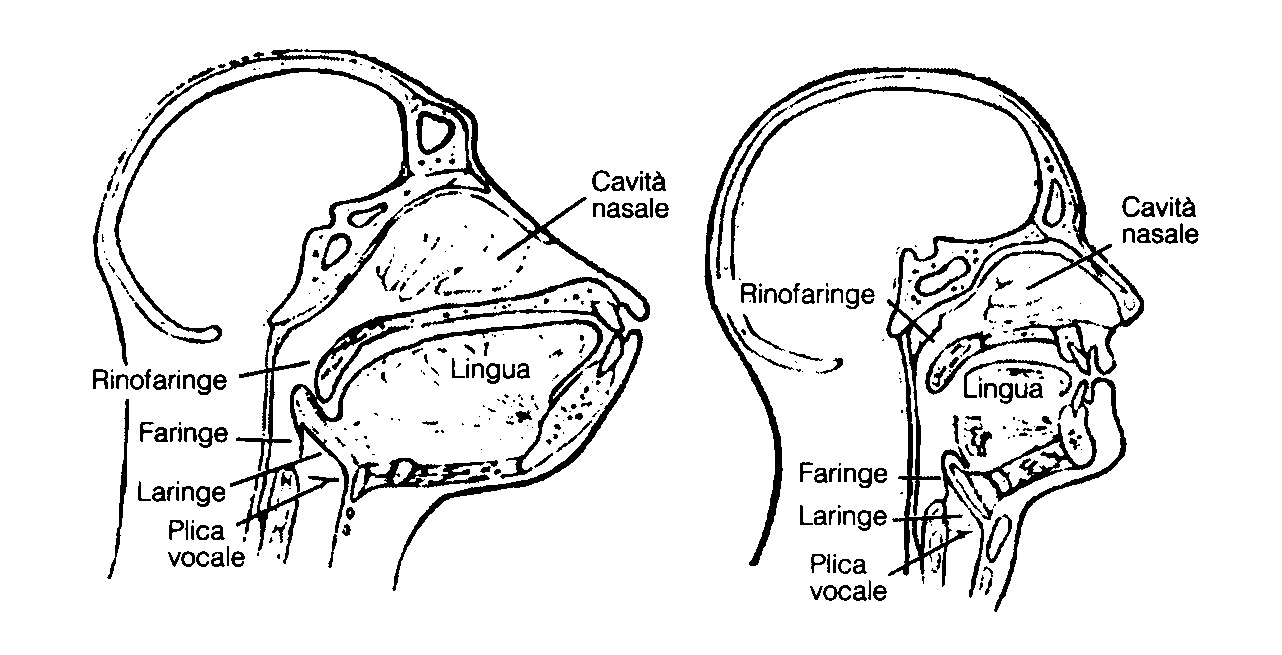
\includegraphics[width=0.4\linewidth]{lezione_3/imgs/0016.jpg}
\end{figure}


\section{40000 - 4000 a.c | Arte grafico-pittorica | Preistoria}
L'uomo delle caverne rappresentava e comunicava attraverso disegni complessi e "realistici" (vedi Lascaux, Altamira, Chauvet), per cui erano necessarie abilità artistiche e molto tempo per essere realizzati, oltre al fatto che venivano realizzati in condizioni sfavorevoli: grotte, poca illuminazione, freddo, \hl{strumenti precari} e poco precisi.
    \subsection{Il significato}
    E' luogo comune, perchè è ciò che si è sempre pensato e tramandato, pensare che le pitture, spesso raffiguranti scene di vita quotidiana, caccia ed in generale tematiche legate al mondo animale, fossero una sorta di \hl{rito propiziatorio}, per sperare in battute di caccia abbondanti e di successo.
    \\\\In realtà, più recentemente, si è sviluppata una teoria più profonda, giustificata da prove tangibili, che vede queste pitture come parte di \hl{riti di passaggio}.
    \subsubsection{Narrazione educativa}
    Facendo un piccolo passo indietro, gli uomini non vivevano nelle caverne, erano solo un luogo di ritrovo; da questa considerazione, aggiungendo il fatto che in queste grotte sono state ritrovate \hl{impronte di bambini accanto a quelle di adulti}, si è giunti a teorizzare che queste pitture potessero essere \hl{una narrazione educativa per i giovani, per insegnare loro le dinamiche della natura selvaggia oltre le zone protette del villaggio }
    \subsubsection{Phanteon di divinità animali}
    Altre teorie, inoltre, aggiungono a quanto detto l'idea che queste raffigurazioni animali possano creare una sorta di \hl{Phanteon di divinità}.

    L'uomo, infatti, al tempo era nettamente inferiore rispetto agli animali, sia in termini numerici, sia a livello di forza. L'animale, principalmente il predatore, veniva temuto dall'uomo, in quanto capace di ucciderlo.

    Allo stesso tempo, però, questa sua superiorità veniva ammirata e, probabilmente, proprio le pitture servivano per raccontare questo mondo animale; \hl{la narrazione veniva fatta da un individuo dotato della capacità di entrare in contatto}, spiritualmente e mentalmente parlando, con questo mondo: \hl{lo sciamano}.

    E anche di questa figura abbiamo delle prove: ci sono diverse pitture e disegni che raffigurano un \hl{individuo mezzo uomo, mezzo animale}.
\begin{mdframed}[style=mystyle,frametitle=Curiosità]
     Anche Picasso, ammirava ed era affascinato dalle pitture rupestri (in particolare quelle di Altamira) perchè le vedeva come un dipinto dell'infanzia dell'umanità, che riportavano all'identità di quest'ultima. Dalla pimordialità delle pitture, Picasso prende spunto e le usa come punto di riferimento per esprimersi come artista. Si nota quindi come queste pitture hanno condizionato la storia dell'arte nel tempo
    \end{mdframed}

    \subsection{Grotte di Chauvet | Video RAI}
    siamo nel sud della Francia, Provenza, grotta di Chauvet, scoperte nel \textbf{\textit{1994}}. Queste grotte rappresentano il sito con le pitture rupestri più antiche, \hl{risalenti a circa 35000 anni fa}
\\\ Attraverso la visiione e l'analisi di queste pitture è possibile risalire a diversi aspetti della vita dell'uomo delle caverne, delle sue abitudini e delle sue credenze.
\\\\La grotta è strutturata su più "livelli", ognuno dei quali è caratterizzato da un colore: c'è ad esempio la \hl{zona rossa}, con le pitture raffiguranti mani "in negativo", oppure la \hl{zona nera}, con raffigurazioni animali
    \subsubsection{Culto degli animali}
    Proprio nella zona nera è possibile visionare la parte più interessante ed elaborata della grotta: sono infatti presenti \hl{numerosissime scene di caccia}, raffiguranti animali di diversa natura: \hl{orsi, cavalli, bisonti, leoni...}.
    \\\\ E' però curioso notare come \hl{la totalità delle scene di caccia non presentano l'uomo come componente}; questo è dovuto al fatto che, come già detto in precedenza, l'uomo del tempo era nettamente inferiore all'animale, e perciò questi disegni sono come una sorta di "ammirazione" del mondo animale. Anche del loro potenziale significato si è già parlato: non si tratta di riti propiziatori, bensì venivano usati come spiegazioni del mondo selvaggio nei \hl{riti di passaggio} per le nuove generazioni (lo dimostrano le impronte di bambini ritrovate); sono quindi un \hl{pantheon di divinità animali}
    \subsubsection{Movimento e prospettiva}
    Altrettanto interessante è la capacità degli uomini del tempo di saper realizzare, a modo proprio, prospettiva, profondità e movimento.

    Si parla di 35000 anni fa, eppure l'uomo, attraverso particolari disposizioni o "giochi grafici" (tipo bisonte con 6 zampe che, in base alla luce che lo "colpiva", dava l'idea del movimento)
    \begin{figure}[H]
    \centering
    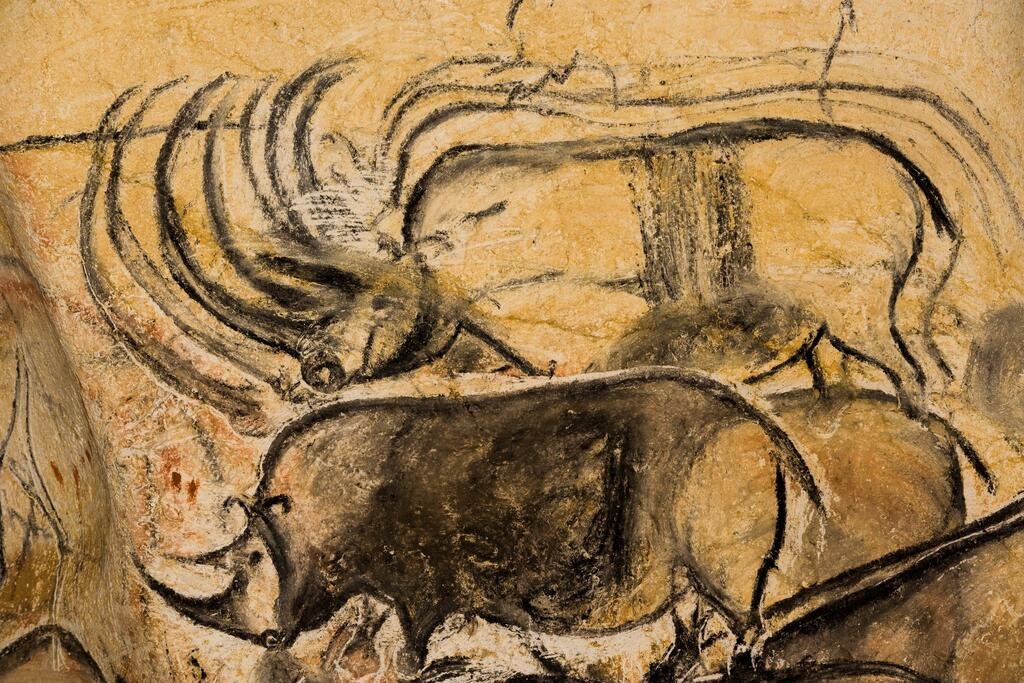
\includegraphics[width=0.4\linewidth]{lezione_3/imgs/la-grotta-chauvet-il-piu-antico-esempio-di-arte-preistorica-del-mondo-prende-vita-con-la-realta-virtuale_07.jpg}
\end{figure}
    
\section{3500 a.c | Pittogrammi}
Sulla base delle pitture rupestri si è poi passato a semplificare i tratti, approdando ai cosiddetti \hl{pittogrammi}: maggior velocità di rappresentazione e maggior stilizzazione sono i tratti distintivi.
    \subsection{Il significato}
    i pittogrammi hanno come \hl{significato ciò che rappresentano}: non sono simboli (come le lettere), bensì sono disegni in cui si può definire un "soggetto/oggetto" (un cervo, un sole...).
    \subsubsection{La componente orale}
    Un limite dei pittogrammi, però, era la necessità di \hl{associare la componente scritta a quella orale}: non bastava, infatti, creare i pittogrammi, ma serviva anche comunicarne il loro significato gli altri

\section{3000 a.c | Ideogrammi | Egizi, Maya, Aztechi e Cinesi}
{\huge \textit{Migliaia di combinazioni}}\\\\
Dalla scrittura pittografica si è poi passati agli \hl{ideogrammi}, la cui principale forma che conosciamo sono i \hl{geroglifici}.

Di fatto gli ideogrammi nascono dall'\hl{unione di diversi pittogrammi che, uniti in sequenza, conferiscono un significato più ampio}.
\\\\Al tempo degli Egizi, i geroglifici venivano usati principalemnet per \hl{testi sacri}, o eventualmente per \hl{narrare le gesta del faraone} (che per di fatto era una divinità...)

\subsection{Egizi}
\\\\I geroglifici rimanevano comunque una tipologia di scrittura molto complessa, che richiedeva molto tempo per essere padroneggiata e la stesura dei testi era lunga; veniva infatti demandata a una figura professionale, lo \hl{scriba}, che lo faceva di mestiere.

\begin{figure}[H]
    \centering
    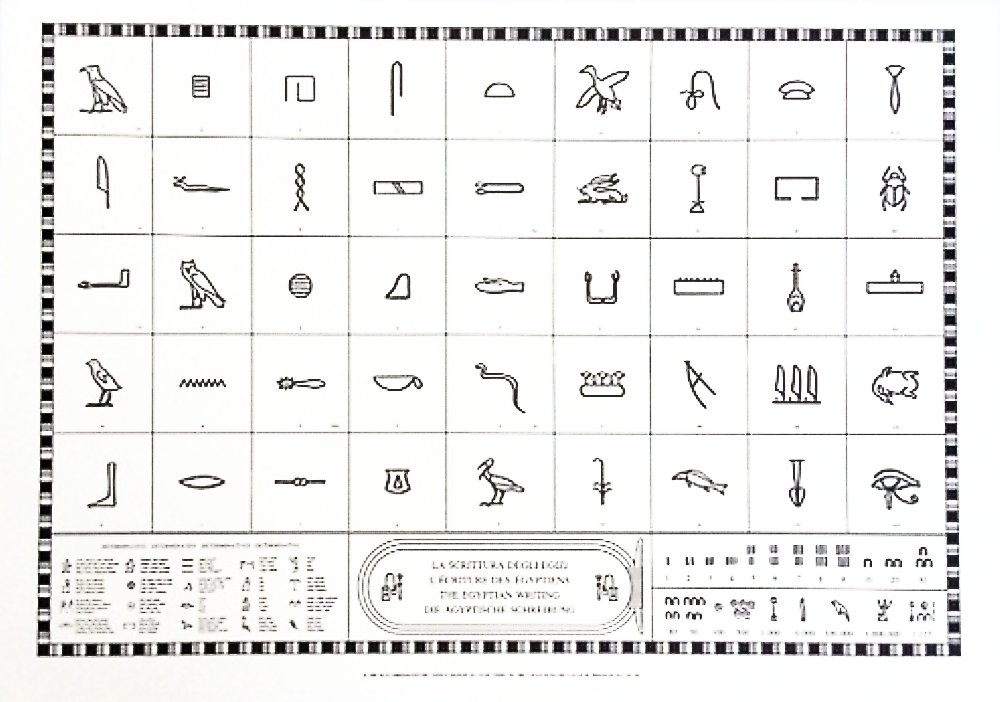
\includegraphics[width=0.4\linewidth]{lezione_3/imgs/61Ucl1IMomL.jpg}
\end{figure}

    \subsubsection{Scritture demotiche e ieratiche}
    Proprio per la sua complessità, gli stessi Egizi si rendono conto che per la gente comune era completamente inutile avere una scrittura così complessa; periò vengono introdotte due nuove tipologie di scrittura:
    \begin{itemize}
        \item \hl{demotiche}: destinate \hl{alla gente comune, le fasce basse} 
        \item \hl{ieratiche}: destinate \hl{a artigiani, architetti..., classe lavoratrice}
    \end{itemize}
    Entrambe le nuove scritture erano caratterizzate da \hl{maggior velocità di scrittura e apprendimento} in quanto \hl{costituite da segni molto semplici}.
    
    Esse permettevano la comunicazione tra il popolo, anche e soprattutto di \hl{tematiche svincolate dalla vita religiosa}, ma più orientata alle \hl{tematiche quotidiane e pratiche}. Si arriva quindi ad un enorme traguardo: \hl{la scrittura non è più circoscritta ad una piccola elite}

    
    \subsection{Maya e Aztechi}
    Sulla decifrazione degli ideogrammi maya e aztechi ci sono ancora oggi molti dubbi circa la collocazione temporale, il loro significato e i loro campi di utilizzo.

    Specialmente per quelli maya, non si è ancora capito se venissero usati, come per gli Egizi, per un uso strettamente legato alla religione, oppure per uso comune
    \subsection{Cinesi}
    La storia degli ideogrammi cinesi è millenaria. Prima degli ideogrammi, infatti, la scrittura cinese era basata su pittogrammi, per poi semplificarsi a ideogrammi.

    E' però curioso notare come il numero di ideogrammi, ad oggi, in uso è di circa 14000 se consideriamo un vocabolario completo!

    Esistono inoltre diversi \hl{stili} di ideogrammi cinesi:
    \begin{itemize}
        \item \hl{ufficiale}, ora chiamato \hl{regolare}: quello usato anche in tipografia
        \item \hl{delle erbe}: è sostanzialmente lo stile calligrafico corsivo
    \end{itemize}


\section{3000 a.c | Scrittura fonetico sillabica | Sumeri}
{\huge \textit{Centinaia di combinazioni}}\\\\
La scrittura, nella sua evoluzione, passa anche per la \hl{scrittura cuneiforme} che, di fatto, è coesistita assieme ai geroglifici. 

Si chiamava cuneiforme perchè, attraverso lo \hl{stilo a sagoma triangolare} usato per incidere, il tratto lasciato risultava proprio a forma di cuneo. 
\\\\
Con i Sumeri, ed in generale con le civiltà della mezzaluna fertile, \hl{cambia il modo di intendere la scrittura}: se gli  ideogrammi erano disegni specifici che avevano lo scopo di richiamare alla mente il significato. ora invece c'è un \hl{associazione simbolo/segno astratto -> suono}.

Questo tipo di scrittura è detta di tipo \hl{fonetico sillabico}, dal momento che \hl{ ogni cuneo/simbolo rappresentava una sillaba}, e nello specifico \hl{la prima sillaba della parola corrispondente all'immagine rappresentata dal segno}

\begin{figure}[H]
    \centering
    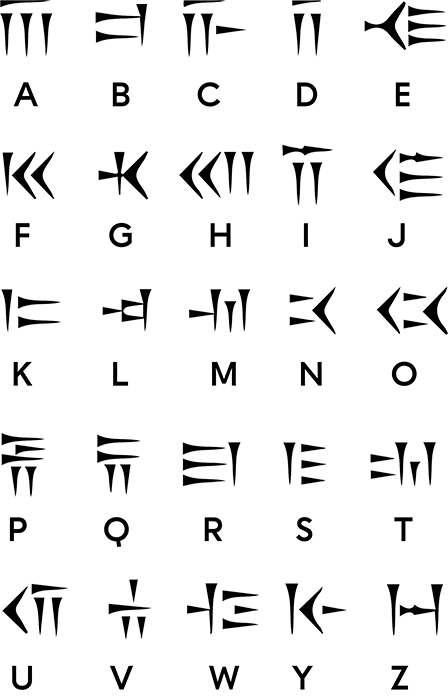
\includegraphics[width=0.3\linewidth]{lezione_3/imgs/tabellaok.png}
\end{figure}

\section{1300 a.c | Sistema alfabetico | Fenici}
{\huge \textit{22 lettere}}\\\\
Fenici, abili navigatori e commercianti, non collocabili geograficamente in maniera precisa in quanto avevano diverse colonie nel Nord-Africa; navigando per ragioni commerciali, entrano in contatto con diverse popolazioni e culture. 

\hl{Hanno quindi bisogno di un metodo di scrittura rapido e efficace per la registrazione di scambi/acquisti...}. Di conseguenza, i Fenici sono i primi che creano di fatto un \hl{primo alfabeto singolo simbolo->singolo suono/pronuncia}, che rappresenta un progresso in termini di rapidità di scrittura.
\\\\
In particolare, per ottenere le varie lettere dell'alfabeto, i Fenici, \hl{partendo da parole complete }(come \textbf{\textit{aleph}}, ossia bue) \hl{ne prendono l'iniziale; per attribuire il simbolo grafico, poi, partono dal pittogramma raffigurante la parola e ne creano una stilizzazione}

\begin{figure}[H]
    \centering
    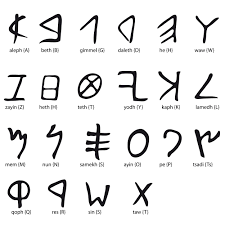
\includegraphics[width=0.3\linewidth]{lezione_3/imgs/images.png}
\end{figure}

\section{900 a.c | Alfabeto greco | Grecia}
{\huge \textit{24 lettere}}\\\\
Il popolo che, basandosi su quanto fatto dai Fenici creando un vero alfabeto completo è quello dei Greci.
\\\\
Avendo comunque un bagaglio di conoscenze ed esperienze matematiche, filosofiche..., i Greci riescono a rendere ancora più pensato e funzionale l'alfabeto introdotto dai Fenici.
Infatti, basandosi su forme quali \hl{triangolo, quadrato e cerchio} (considerate forme perfette secondo la geometria), i Greci creano l'\hl{alfabeto greco}; graficamente e geometricamente più bilanciato, preciso e regolare.

Inoltre, i Greci cambiano anche il verso di scrittura: da \hl{sistema sinistrorso} (usato anche dai Fenici), si passa a quello \hl{bustrofedico} (alternando sinistrorso e destrorso nelle varie righe), per poi approdare definitivamente al \hl{sistema destrorso}.

\begin{figure}[H]
    \centering
    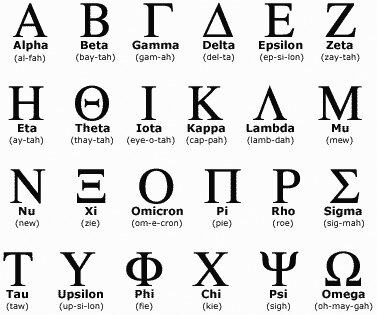
\includegraphics[width=0.3\linewidth]{lezione_3/imgs/6006_Una-passeggiata-nel-greco-antico.jpg}
\end{figure}

\section{400 a.c | Alfabeto etrusco | Etruschi}
{\huge \textit{20 lettere}}\\\\
Dall'influenza dei Greci, anche gli Etruschi utilizzano e creano un loro alfabeto, sempre sulla base di quello greco.

Gli Etruschi, però, ritornano al sistema sinistrorso (dx -> sx)
\\\\
Chiamati anche \hl{popolo delle lettere}, gli Etruschi davano quasi una \hl{valenza magica} alla scrittura e alle lettere, tanto che \hl{venivano usate per ornare le tombe}
\begin{figure}[H]
    \centering
    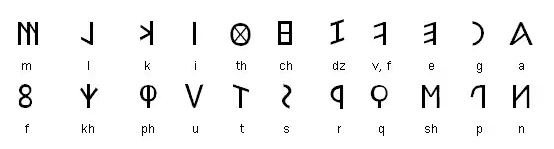
\includegraphics[width=0.5\linewidth]{lezione_3/imgs/alfabeto-etrusco1.png}
\end{figure}
\section{Monumentali, quadrate e rustiche | Romani}
\subsection{Capitali monumentali romane}
{\huge \textit{23 lettere}}\\\\

I Romani, influenzati dal popolo etrusco e affascinati dal popolo greco, adottano il sistema alfabetico, facendo però un ulteriore passo avanti: creano dei veri e propri \hl{canoni geometrici} che l'intera schiera di lettere facenti parte dell'\hl{alfabeto latino} (questo è il nome del nuovo alfabeto di 23 lettere) deve rispettare.

\begin{mdframed}[style=mystyle,frametitle=Curiosità]
    La scrittura, per i Romani rappresenta, principalmente nel periodo dell'impero, una sorta di \hl{uniformazione linguistica}: tutti i documenti scritti che circolavano tra le province, erano scritti tutti usando l'alfabeto latino da loro ideato
    \end{mdframed}

La \hl{colonna traiana} è un spesso preso come riferimento per rendersi conto di come questi nuovi caratteri siano stati fin da subito adottati nella realizzazione di opere-simbolo della civiltà romana; il fatto che fossero studiati e progettati nei minimi dettagli li rendeva praticamente perfetti e utilizzabili per opere monumentali.
    \subsubsection{Caratteristiche delle lettere monumentali romane}
    Come detto, i Romani, le loro lettere, sono pura geometria! Non è la semplice geometria, per che rende queste lettere pressoché perfette, equilibrate, 
    Ci sono infatti una serie di peculiarità legate a questo alfabeto:
    \begin{itemize}
        \item introduzione delle \hl{grazie}: di "prolungamenti"/piedini alle estremità delle aste delle lettere; conferiscono \hl{stabilità}
        \item \hl{modularità del tratto}
        \item incisione con \hl{sezione triangolare}: sostituisce quella a sezione quadrata; conferisce \hl{maggior restistenza all'usura} e \hl{crea giochi di luce} accattivanti
        \item \hl{struttura a moduli}: le lettere venivano progettate partendo da una \hl{griglia 4 moduli x 4} in base poi a quanti moduli orizzontali venivano occupati, si potevano avere:
            \begin{itemize}
                \item 2x4: lettere strette
                \item 3x4: lettere medie
                \item 4x4: lettere larghe
            \end{itemize}
    \end{itemize}

    Ovviamente, queste caratteristiche erano state pensate per conferire all'alfabeto \hl{estrema funzionalità e al tempo stessa maestosità estetica} per rendere l'impero riconoscibile e magifico agli occhi esterni.
    Infatti, prendendo per esempio le grazie, danno eleganza e stabilità ai caratteri, ma allo stesso tempo sono state pensate per facilitare la creazione delle bozze e l'incisione (vedi ordinator e lapicida più avanti).

    \begin{figure}[H]
    \centering
    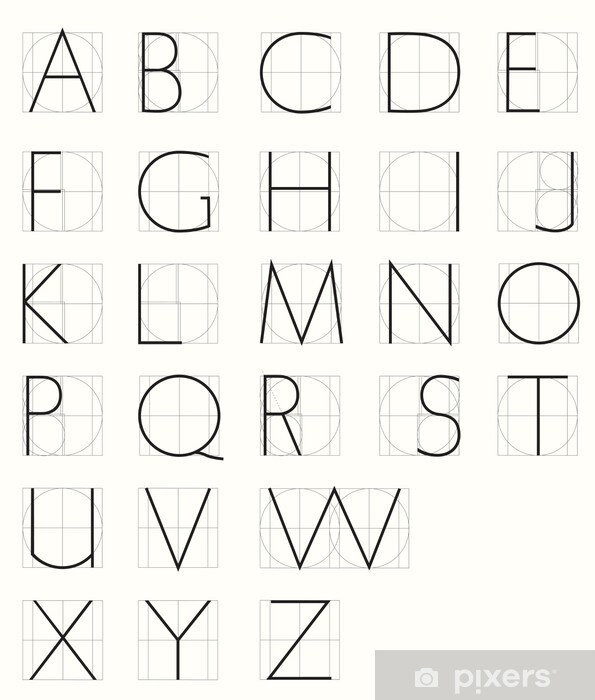
\includegraphics[width=0.4\linewidth]{lezione_3/imgs/carte-da-parati-capitali-romane-monoline-con-griglia-geometrica.jpg.jpg}
\end{figure}
    \subsubsection{Ordinator e lapicida}
    Come già detto, le novità introdotte dai Romani sulle lettere sono pensate anche per ragioni di funzionalità.
    Nello specifico, grazie, modularità del tratto e sezione triangolare sono la conseguenza di come veniva gestita la creazione delle incisioni.

    Erano infatti necessarie due figure per la realizzazione:
    \begin{itemize}
        \item \hl{ORDINATOR}: colui che realizzava i bozzetti delle lettere sulla pietra. Utilizzava un \hl{pennello a punta piatta, la \textbf{\textit{SPATOLA}}}, iniziava la bozza della lettera facendo un movimento rotatorio del pennello, formando quindi la \textbf{\textit{grazia}}
        \item  \hl{LAPICIDA}: colui che incideva la pietra. Grazie alle grazie create dall'ordinator, poteva essere facilitato al momento del primo colpo di scalpello, proprio perchè la grazia è un punto molto fine, e quindi ottimale per inserire lo scalpello
    \end{itemize}

    Questa operazione, nel suo complesso, richiedeva una maniacale precisione e delle tempistiche molto lunghe; questa è la motivazione per cui i Romani tendono a \hl{accorciare le parole e le frasi}
    

\begin{mdframed}[style=mystyle,frametitle=Roma come i moderni brand]
     a suo modo anche l'impero, con i suoi simboli, i suoi motti, il suo colore, le monete, i monumenti, le piante delle città, sviluppa una identità visiva che rendeva iconico l'impero e permette di avere una uniformità in tutte le province
    \end{mdframed}

\subsection{Capitali quadrate | Romani}
i Romani, però, si rendono conto che le capitali monumentali non sono la scrittura ideale per i contesti quotidiani, data la complessità e il rigore che questa scrittura richiede; introducono quindi le cosiddette \hl{capitali quadrate}, caratterizzate da:
\begin{itemize}
    \item \hl{sistema a griglie/moduli} meno rigido delle monumentali (\hl{a base quadrata})
    \item \hl{grazie}, ma meno rifinite rispetto alle monumentali
    \item solo \hl{lettere maiuscole}
    \item altezza regolare (tranne F e L)
\end{itemize}
Risultano quindi essere una semplificazione delle monumentali, usato comunque per almeno 3 secoli
\subsubsection{Angolo e posizione scrittura scomodo}
Nonostante fosse un carattere più adatto per la stesura di testi in maniera più rapida, la \hl{posizione e angolo di scrittura (quasi orizzontale) } rendevano la scrittura poco comoda e fluida per la mano. Di conseguenza, se inizialmente veniva usato per testi lunghi e importanti, è poi stato adottato solo per titoli o lettere decorate.
\begin{figure}[H]
    \centering
    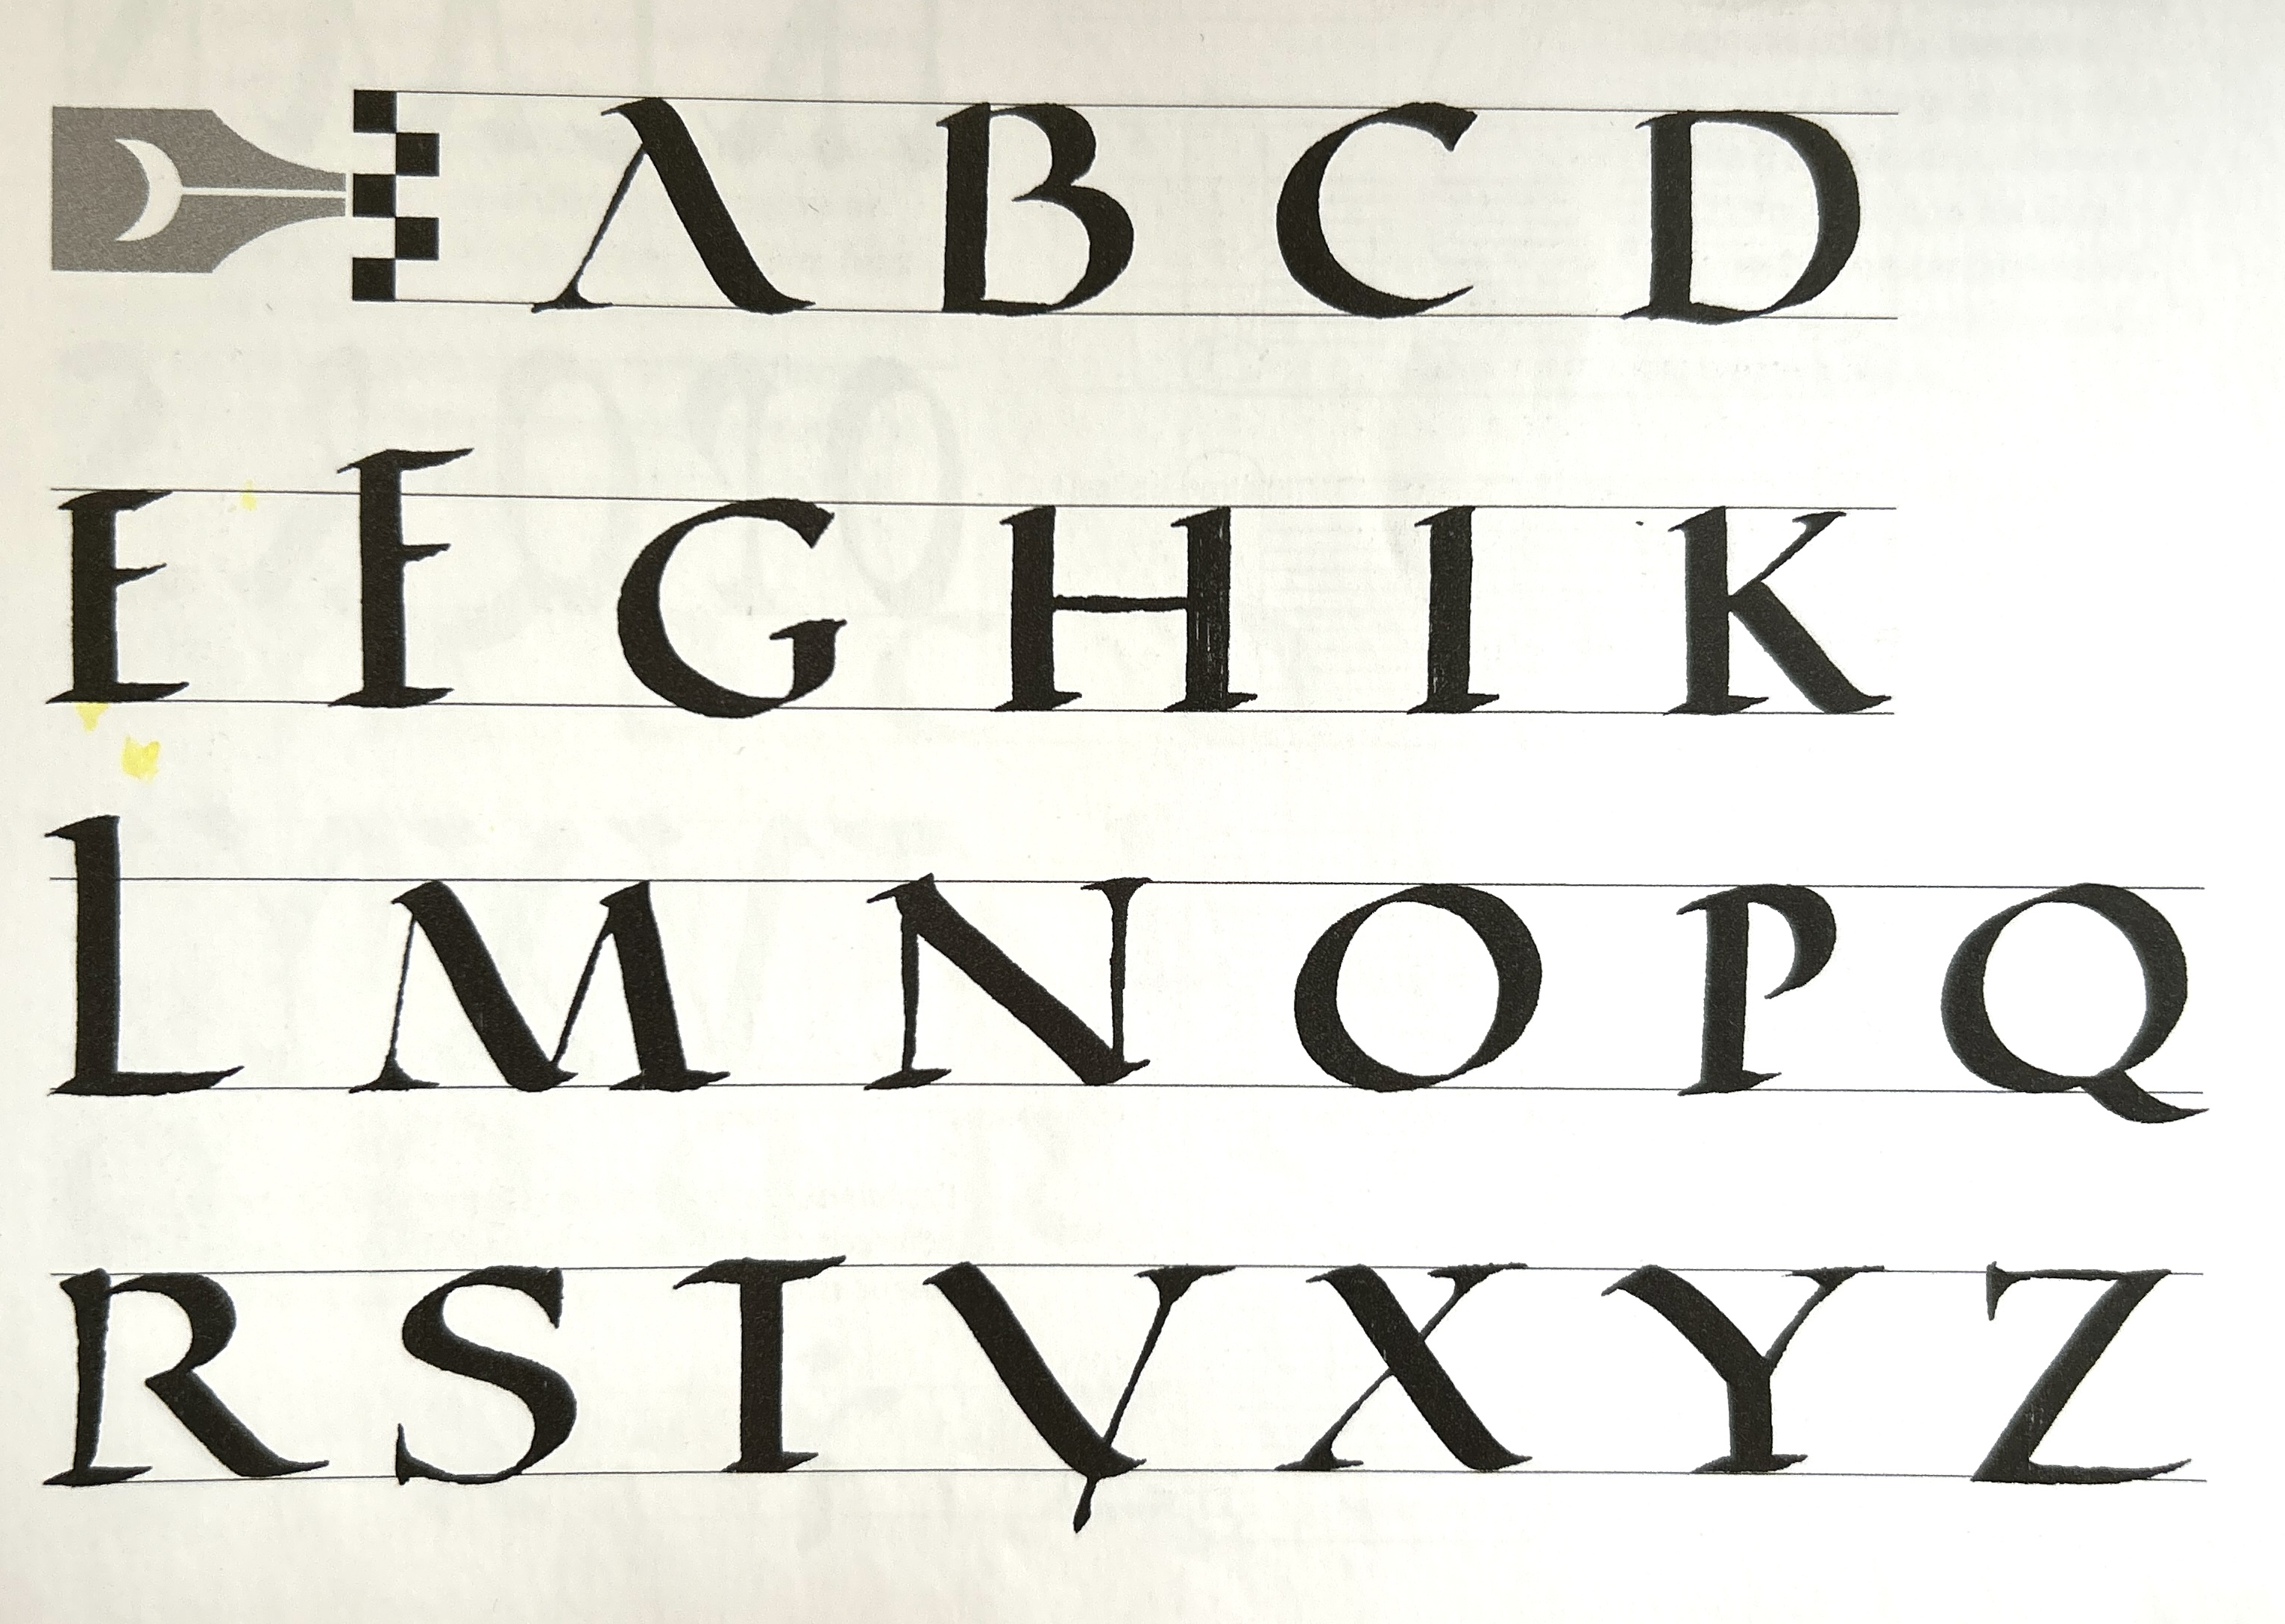
\includegraphics[width=0.3\linewidth]{lezione_3/imgs/cap_quadrata.jpg}
\end{figure}
\subsection{Capitali rustiche | Romane}
le \hl{capitali rustiche} rappresentano una terza variante della scrittura romana, \hl{ancora più rapida nella stesura rispetto a quella quadrata}; questa è una conseguenza diretta delle peculiarità di questo carattere:
\begin{itemize}
    \item tratto più libero rispetto a quadrate e quindi monumentali
    \item tratto modulare e meno strutturato
    \item lettere più strette rispetto a quadrate e monumentali
\end{itemize}
\begin{figure}[H]
    \centering
    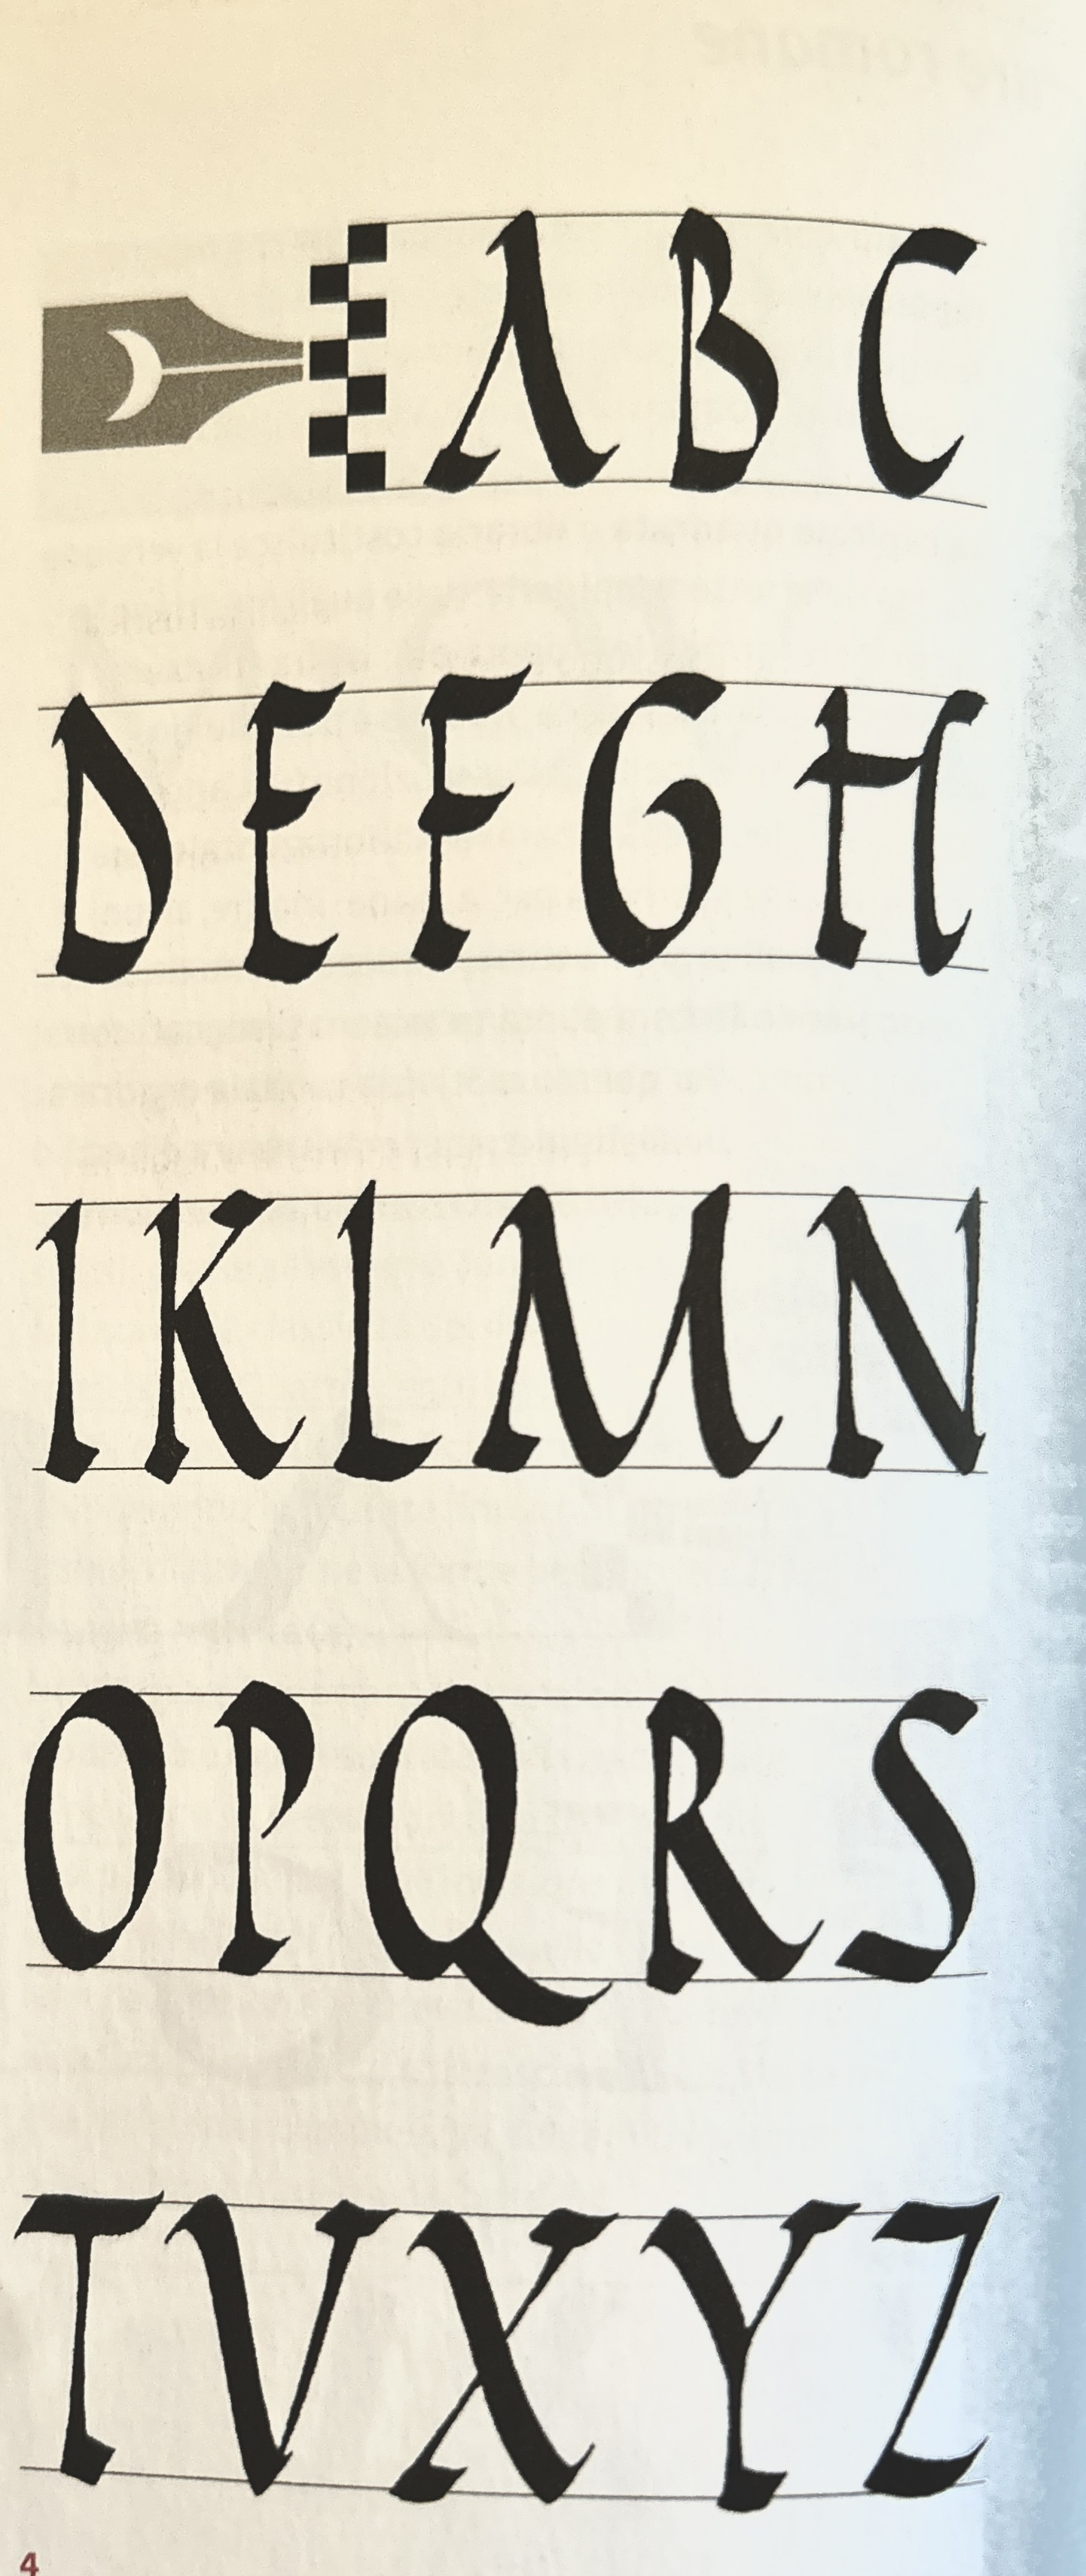
\includegraphics[width=0.2\linewidth]{lezione_3/imgs/cap_rustica.jpg}
\end{figure}

\subsection{Tabellae e Volumen}
Se le monumentali erano associate a supporti quali colonne, monumenti, o più in generale superfici che potevano essere incise, rustiche e quadrate erano usate su supporti molto più portabili e comodi; \hl{la Tabellae} e \hl{il Volumen}.
\\\\
la \hl{tabellae} era una sorta di "quaderno", composto da due tavolette di legno richiudibili ricoperti da uno strato di cera che veniva inciso con uno \hl{stilo}.

La superficie su cui scrivere era poca, motivo per cui questo "costringeva" ad usare metodi di scrittura molto più rapidi rispetto alle monumentali.
\begin{figure}[H]
    \centering
    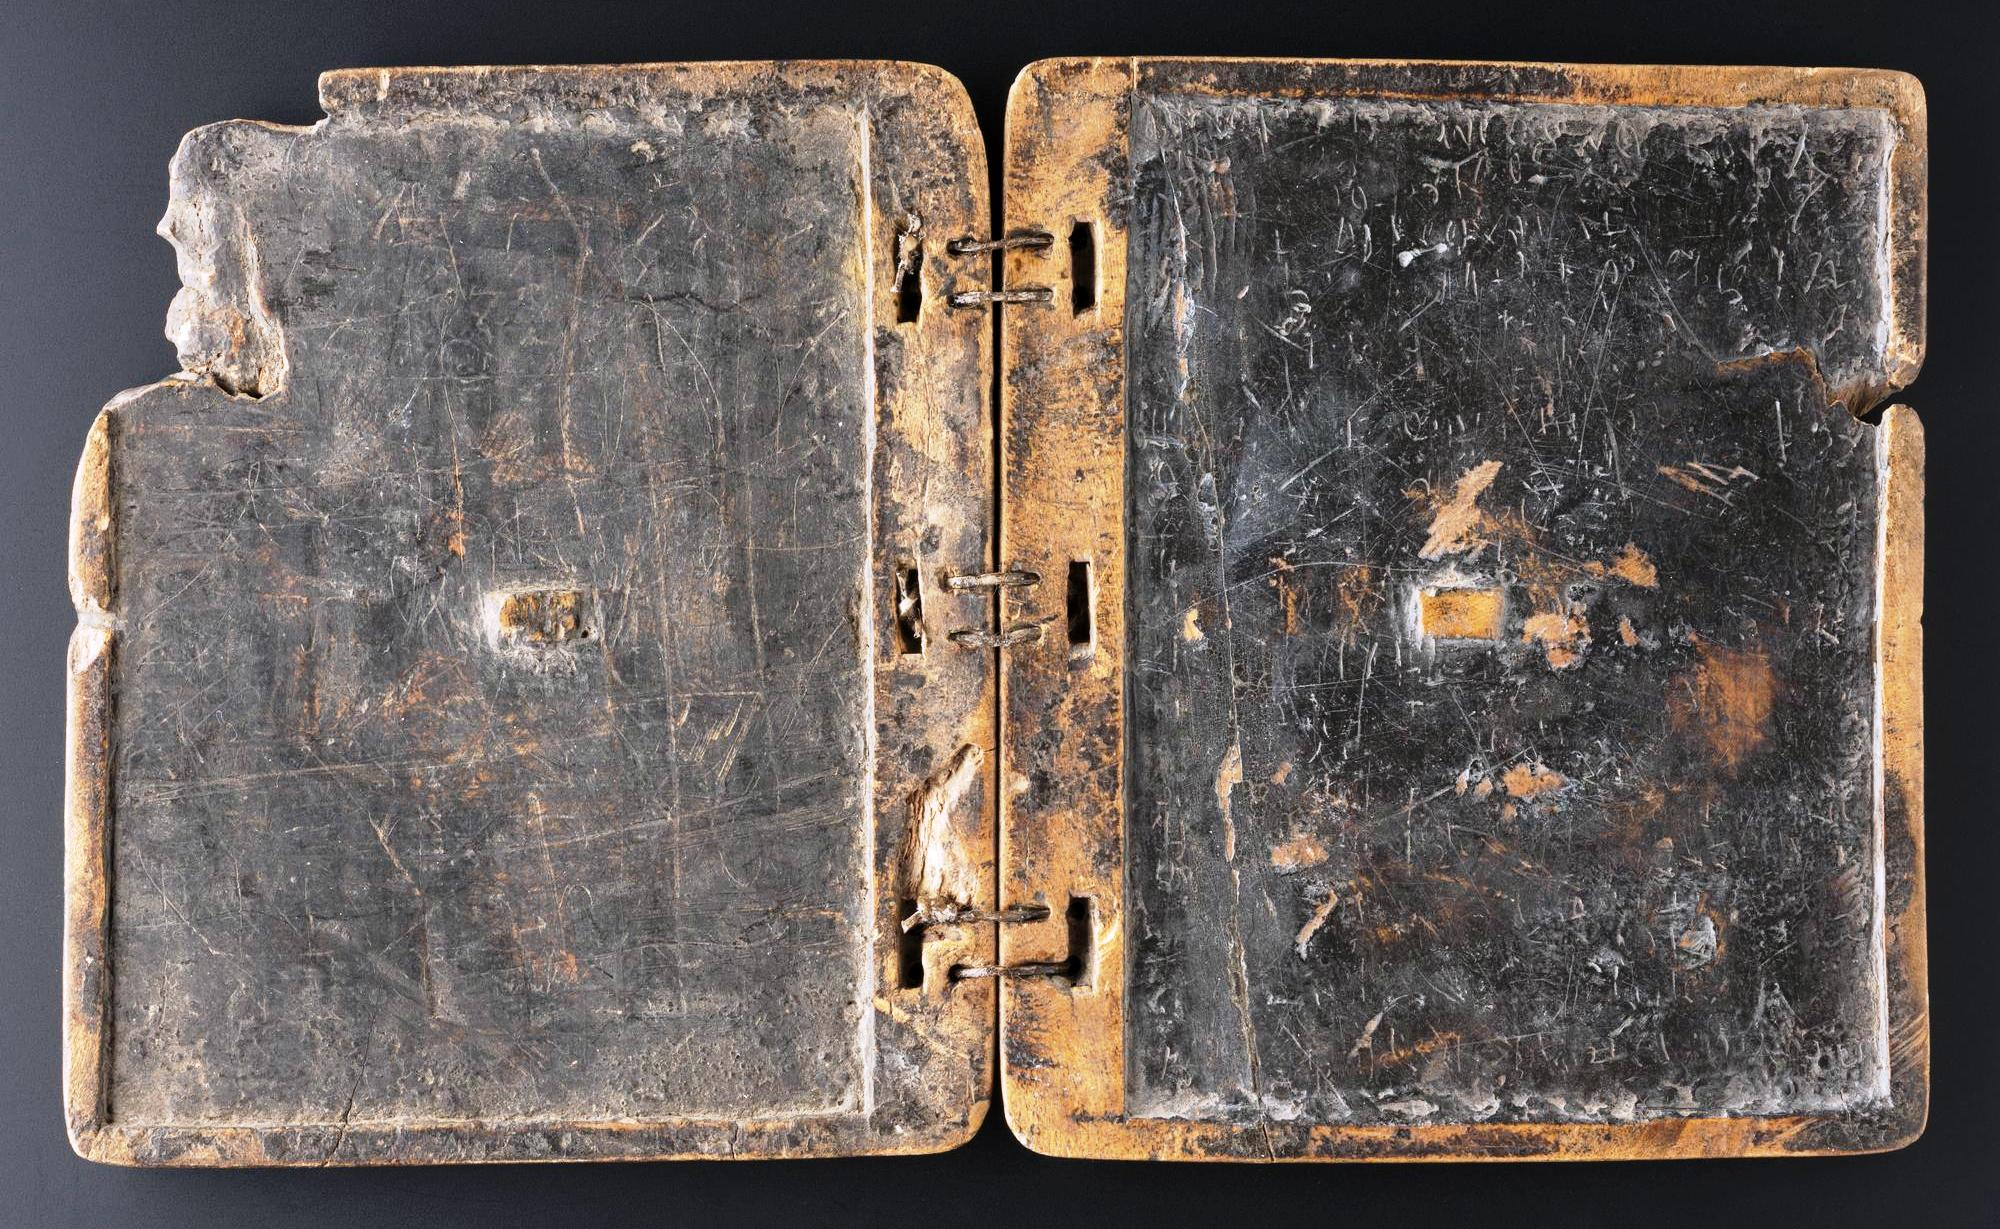
\includegraphics[width=0.3\linewidth]{lezione_3/imgs/varivs_scriptio20b.jpg}
\end{figure}
\\\\
il \hl{volumen}, invece, non era niente altro che un rotolo di papiro che fungeva da "libro"; erano usate infatti diverse tipologie di impaginazioni che permettevano l'organizzazione del testo in modi diversi
\begin{figure}[H]
    \centering
    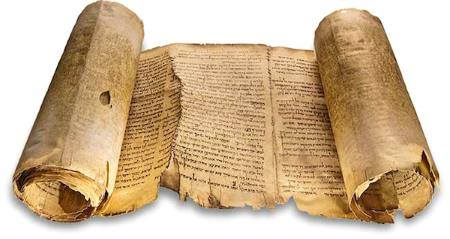
\includegraphics[width=0.3\linewidth]{lezione_3/imgs/17495684_10209129661334783_1817188107_n-1.jpg}
\end{figure}
\section{Scritture medievali}
Con la caduta dell'impero, si ricerca anche delle nuove forme e caratteri facili da usare, funzionali e rapidi. Le monumentali ed in generale le scritture romane non erano ideali data la difficoltà di esecuzione (chi più, chi meno).
\\\\
Si vanno a ricercare quindi forme essenziali e facilmente riconoscibili e scrivibili: il primo esempio che da il via a queste nuove forme di scrittura sono le \hl{onciali}, che sono il punto di partenza per l'identificazione di uno stile che porterà all'\hl{introduzione delle minuscole}.

\subsection{Edward Johnston | Foundational}
Tra di loro i caratteri medievali presentano caratteristiche molto simili, tra cui ad esempio la presenza di un contrasto tra i tratti orizzontali e verticali.
\\\\
il calligrafo \hl{Edward Johnston}, studiando queste caratteristiche comuni dei caratteri medievali (es. onciale, semionciale, beneventata, visigotica...), ne ha definito un carattere chiamato \hl{Foundational}, comprendente tutte le peculiarità principali in un unico carattere.
\subsection{Hann Kamp | schema scritture medievali}
\hl{Hann Kamp}, invece, è stata in grado, attraverso lo studio dei caratteri medievali e sulla base del Foundational, di definire uno \hl{schema/scheletro} all'interno della quale potessero essere inserite tutte le lettere presenti nell'alfabeto
\subsection{Scrittura onciale}
è la prima scrittura che introduce, seppur non in maniera definitiva (solo su alcune lettere), \hl{le minuscole}, ossia quelle lettere che presentano, oltre alla forma base inserita nel rigo, porzioni che fuoriescono da quest'ultimo: le \hl{ascendenti e discendenti}. La minuscola, in linea generale, risulta essere molto più rapida nella stesura del tratto 
\begin{figure}[H]
    \centering
    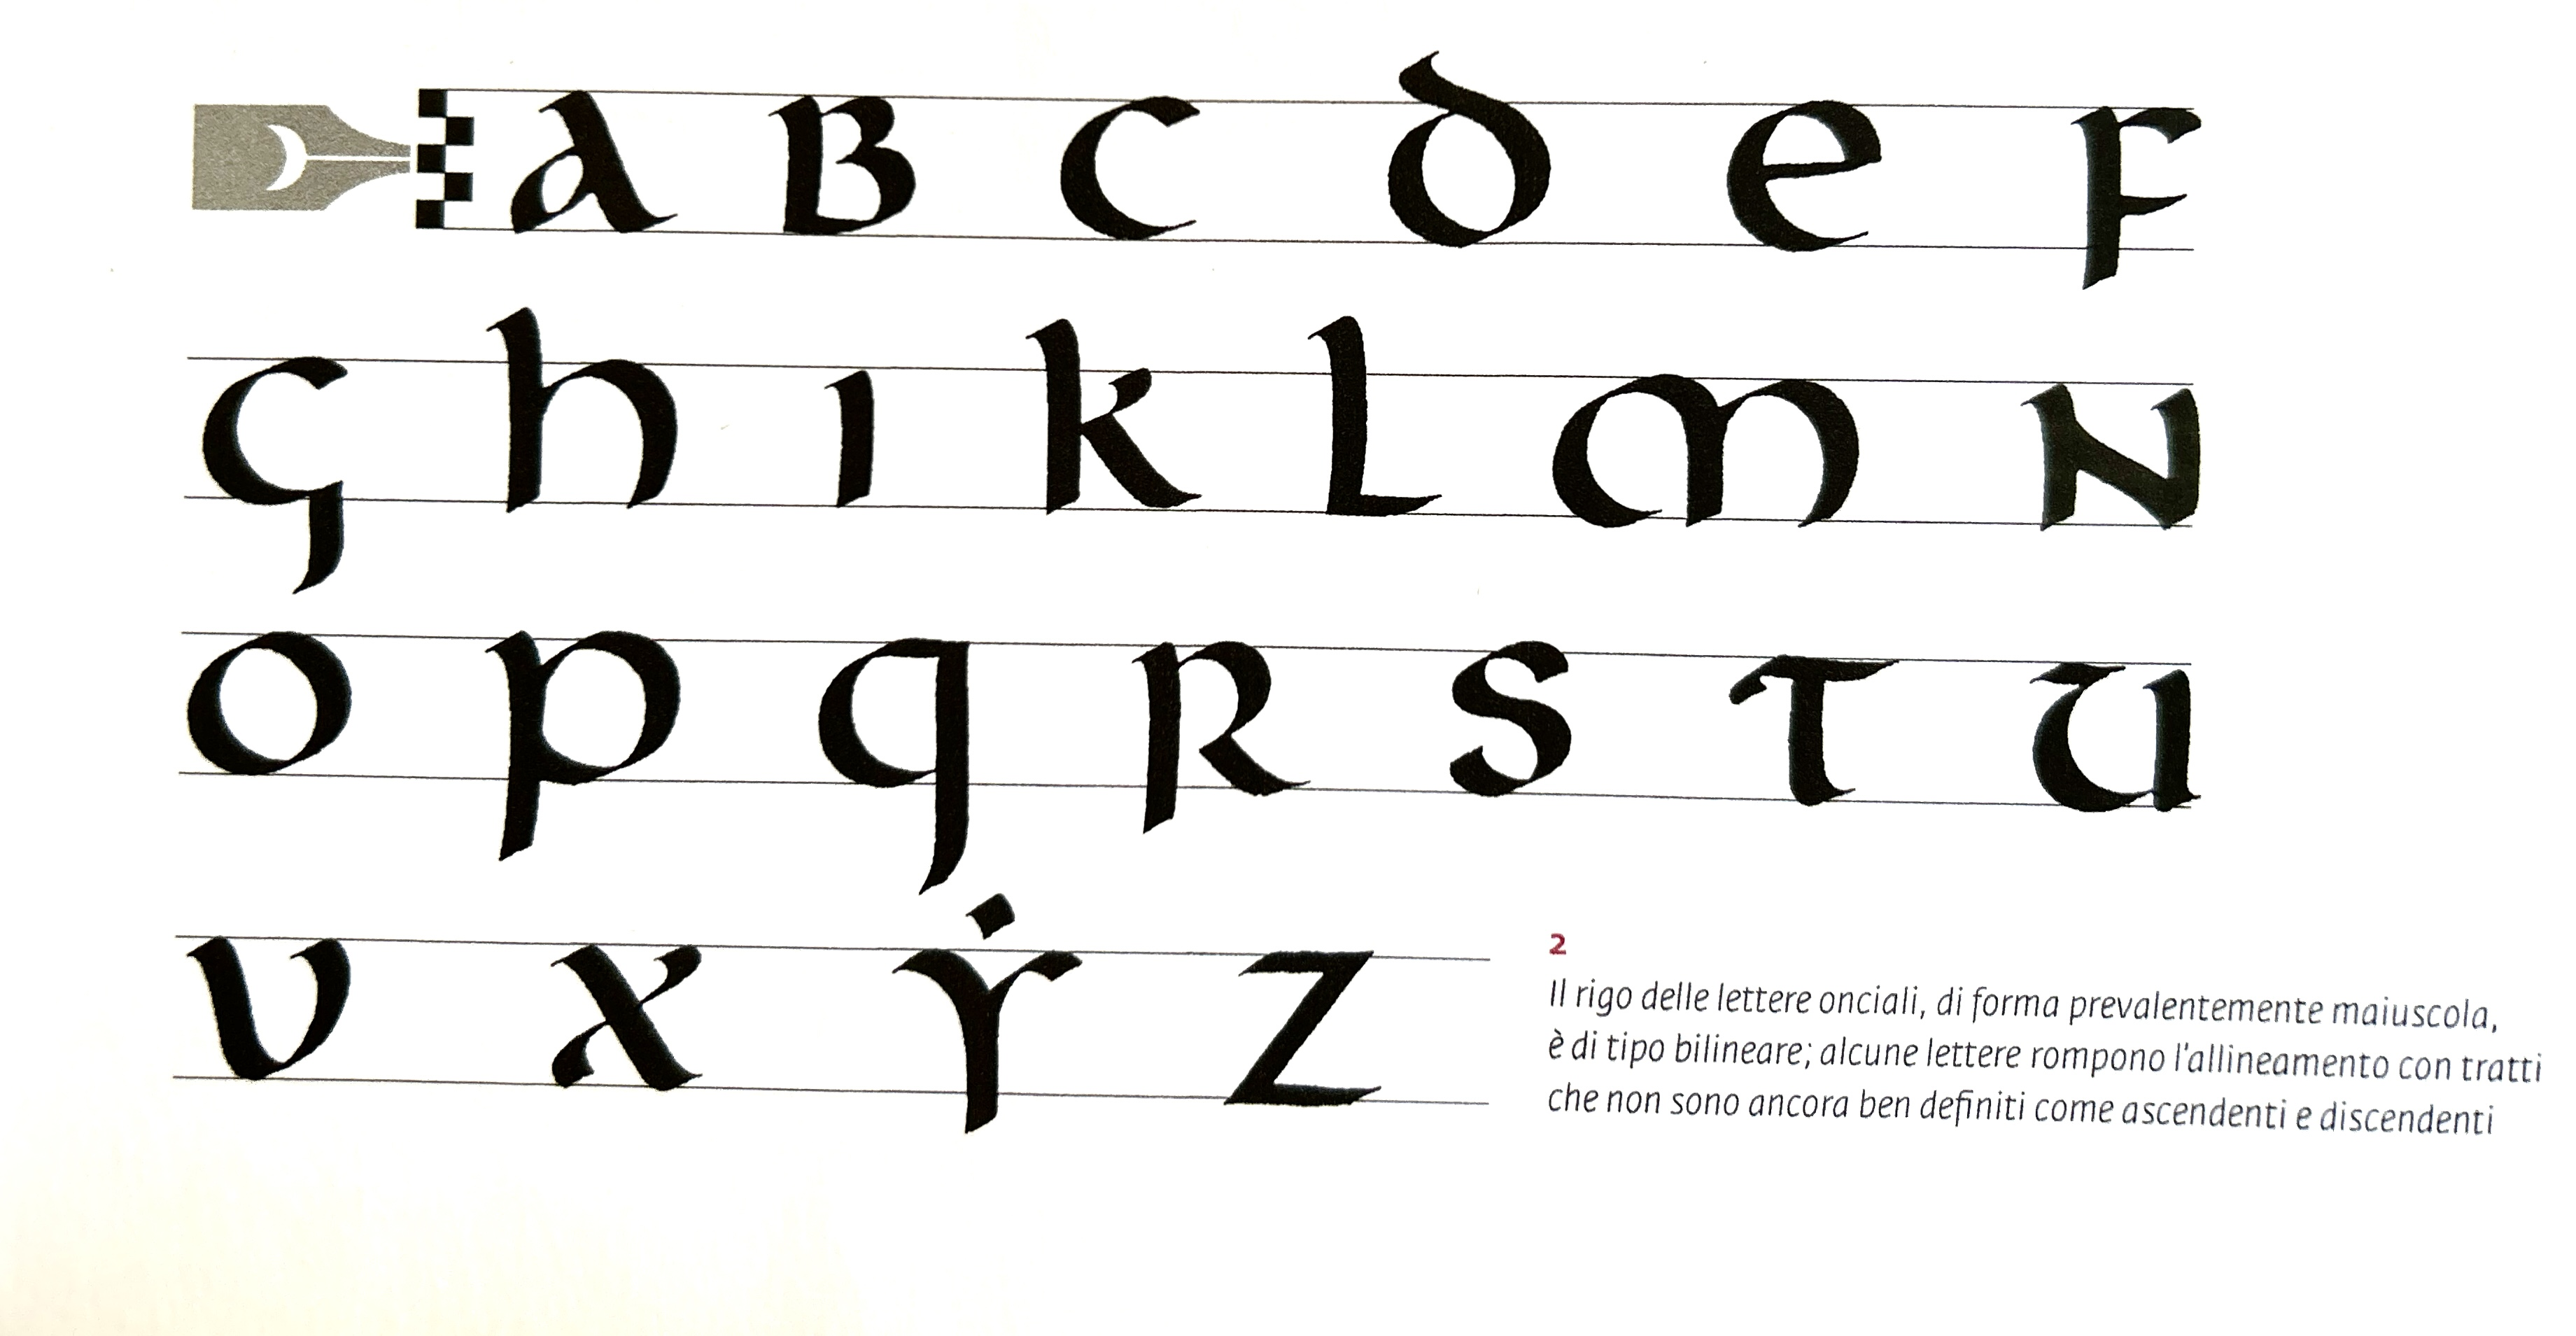
\includegraphics[width=0.4\linewidth]{lezione_3/imgs/onciale.jpg}
\end{figure}
\subsection{Codex: la pergamena}
parallelamente all'introduzione della scrittura onciale, viene introdotta anche la \hl{pergamena} che, in poco tempo, prende piede talmente tanto da sovrastare il papiro.

Rispetto al papiro, infatti, la pergamena:
\begin{itemize}
    \item origine animale e non vegetale
    \item più laboriosa da preparare
    \item prestazioni migliori
    \item meno sensibile alle variabili ambientali/fisiche/atmosferiche
\end{itemize}
\subsubsection{Storia della pergamena}
La pergamena prende il nome dalla città di Pergamo, colpita da un embargo del papiro da parte dell'Egitto.

Questo embargo puntava a rallentare la crescita dell'enorme biblioteca di Pergamo (rivale di quella di Alessandria, che nel passato è stata anche soggetto di un incendio, considerato uno dei più tragici della storia).
\\\\
A Pergamo, quindi, si è dovuto trovare una soluzione per sopperire alla mancanza del papiro, inventando \hl{la pergamena}

\subsubsection{Piegatura e moderna imposition}
La pergamena, oltre ad avere delle peculiarità già descritte che la rendono più adatta rispetto al papiro, presenta una novità: \hl{la piegatura}. Infatti, se il papiro era composto da striscioline vegetali, che limitava la dimensione globale del "foglio", la pergamena, fatta di pelle animale, \hl{poteva avere dimensioni enormi}; di conseguenza l'arrotolamento risultava scomodo per la pergamena.
\\\\
Esistevano diverse piegature (in base alla dimensione della pergamena):
\begin{itemize}
    \item in-folio : in 2
    \item \hl{in-quarto: in 4, quartino}
    \item in-octava: in 8
\end{itemize}
è proprio \hl{il quartino} che è ancora alla base della moderna \hl{imposition} (\textbf{\textit{= gestione e ordinamento delle pagine pre-stampa}}) tipografica.
In tipografia, infatti, \hl{il quartino rappresenta l'unità minima di un foglio piegato}, usato per la realizzazione di volantini, richiudibili...
\begin{figure}[H]
    \centering
    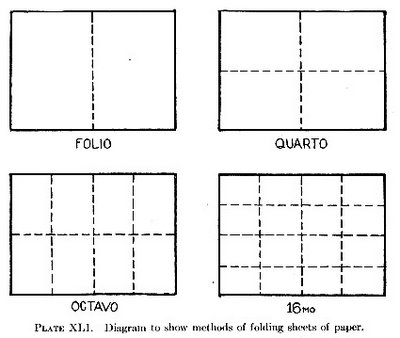
\includegraphics[width=0.5\linewidth]{lezione_3/imgs/Plate41_Printed Book Sheet.jpg}
\end{figure}